\chapter{การออกแบบและวิธีการดำเนินงาน}

\section{การสำรวจความต้องการกับผู้ใช้}
ทางคณะผู้จัดทำได้ทำออกเก็บข้อมูลกับกลุ่มเป้าหมายมาแล้วทั้งหมด 4 ครั้ง โดยแบ่งเป็นการสัมภาษณ์เชิงปริมาณหนึ่งครั้งและเชิงคุณภาพสามครั้ง  โดยมีจุดประสงค์ในแต่ละการสัมภาษณ์ต่างกันเพื่อพิสูจน์ความต้องการของกลุ่มเป้าหมายจนกระทั่งโครงงานของเราได้ปรับตามความต้องการนั้นจนเป็นโครงงานในปัจจุบัน อย่างไรก็ตาม เรายังได้รับข้อมูลที่น่าสนใจเพิ่มเติมโดยสรุป ดังนี้

\subsection{การสัมภาษณ์เชิงปริมาณผ่านแบบสำรวจ}
ทางคณะผู้จัดทำได้ทำแบบสอบถามเพื่อหาอัตราส่วนของพฤติกรรมที่น่าสนใจ โดยได้รับข้อมูลที่สำน่าสนใจดังนี้
\begin{figure}[!h]\centering
    \setlength{\fboxrule}{0.2mm} % can define this in the preamble
    \setlength{\fboxsep}{0.5cm}
    \fbox{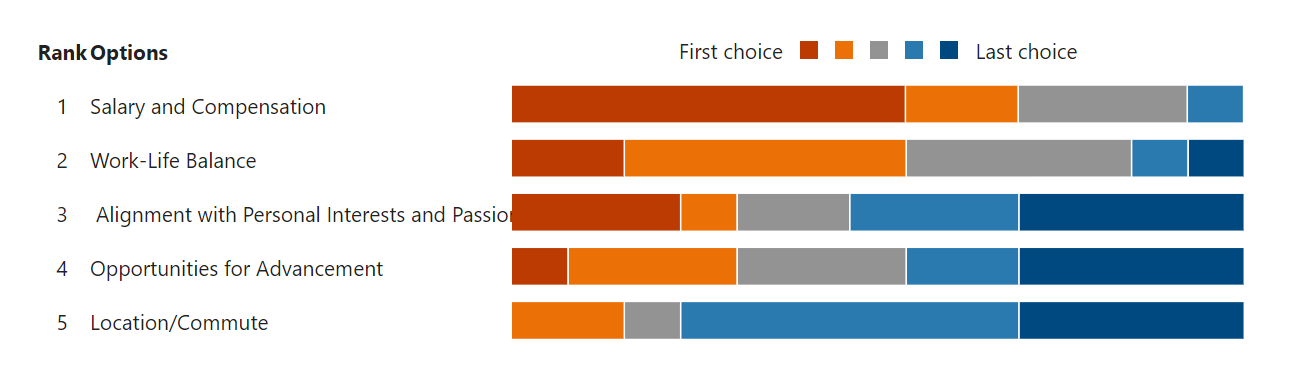
\includegraphics[width=10cm]{./figure/figure_poll.png}}
    \caption{ข้อมูลจากแบบสำรวจเชิงปริมาณ}\label{fig:model4}
\end{figure}
จากข้อมูลในแบบสำรวจข้อนี้ ทำให้ทราบว่าปัจจัยที่มีผลต่อการเลือกสายงานในการทำงานมากสำหรับกลุ่มตัวอย่างก็คือเงินเดือน และความสมดุลของการทำงานกับชีวิตส่วนตัว กล่าวคือกลุ่มตัวอย่างให้ความสำคัญกับความจริงมากยิ่งขึ้น ความมั่นคง หรือเงินเดือนที่สามารถทำให้ดำเนินชีวิตได้อย่างราบรื่น รวมถึงการแบ่งเวลา การพักผ่อนที่เหมาะสมกับการทำงาน โดยมองอาจจะไม่ได้ให้ความสำคัญกับความชื่นชอบมากขนาดนั้น

\subsection{การสัมภาษณ์เชิงคุณภาพผ่านการสัมภาษณ์ตัวต่อตัว}
ทางคณะผู้จัดทำได้ออกสัมภาษณ์กับกลุ่มเป้าหมายแบบตัวต่อตัว และในการสัมภาษณ์แต่ละครั้ง จะสัมภาษณ์ที่จำนวนราว 5 คน ตามหลักการที่กล่าวไปใน [xx] โดยได้รับข้อมูลที่น่าสนใจในแต่ละครั้งมาดังนี้

การสัมภาษณ์เชิงคุณภาพครั้งที่ 1

จุดประสงค์: เพื่อค้นหารากขอปัญหาที่แท้จริงของกลุ่มเป้าหมาย

ข้อมูลสำคัญ: 
\begin{itemize}
    \item กลุ่มเป้าหมายค้นพบความต้องการของตนเองมาจากการได้ลงมือทำจริงเป็นหลัก
    \item ส่วนใหญ่แล้วจะได้ลงมือทำจริงตอนโปรเจ็กต์วิชาเรียนหรือฝึกงาน ซึ่งอยู่ชั้นปีที่ 2 เป็นต้นไปแล้ว
    \item อยากรู้ก่อนเป็นอย่างมาก ว่าในการทำงานจริงต้องมีความสามารถอะไรบ้าง ใช้เครื่องมืออะไร
    \item กลุ่มเป้าหมายรู้สึกว่าอาจรู้ตัวช้าเกินไป หากมีโอกาสพัฒนาตนเองได้เร็วกว่านี้จะดีมาก
\end{itemize}

การสัมภาษณ์เชิงคุณภาพครั้งที่ 2

จุดประสงค์: เพื่อพิสูจน์ความมีคุณภาพของวิธีการแก้ปัญหาที่ออกแบบ


ข้อมูลสำคัญ: 
\begin{itemize}
    \item กลุ่มเป้าหมายอยากได้ตัวช่วยในการทำให้ตนเองสมัครงานได้ง่ายขึ้น โดยหลังการทดลองถามความเห็น พบว่าสิ่งที่ต้องการเป็นหลักคือ การตรวจสอบและยืนยันได้ ว่าเรซูเม่ของตนเองเหมาะสมกับอาชีพที่ตนเองสนใจขนาดไหนแล้ว
    \item กลุ่มเป้าหมายรู้สึกสนใจในฟีเจอร์ช่วยเหลือการค้นหาแหล่งพัฒนาตนเอง เพราะเคยรู้สึกว่าตนเองอาจเริ่มพัฒนาช้าเกินไป เพราะรู้ใจตัวเองในช่วงที่อาจเรียนอยู่ชั้นปีที่ 2-3 แล้ว
    \item การตัดสินใจลงวิชาเรียนค่อนข้างมีจุดขัดใจ เพราะไม่ค่อยมีรีวิวหรือความเห็นของผู้ที่เคยเรียน ถึงแม้เคยมีแหล่งชุมชนที่รุ่นพี่เคยมอบให้ แต่รีวิวส่วนใหญ่จะมีความเก่าแล้ว ทำให้ใช้อ้างอิงได้ยาก
\end{itemize}

การสัมภาษณ์เชิงคุณภาพครั้งที่ 3

จุดประสงค์: เพื่อทดลองนำ prototype ของเว็บแอปไปพิสูจน์ความรู้สึกในการใช้งานกับผู้ใช้

ข้อมูลสำคัญ:
\begin{itemize}
    \item ผู้ใช้ไม่มีปัญหากับการกรอกข้อมูลเรซูเมเพื่อวิเคราะห์ แต่หากมีระบบที่กรอกข้อมูลให้อัตโนมัติผ่านไฟล์ pdf ก็ถือว่าเป็นเรื่องดี
    \item การมีระบบโหวตวิชาที่อยากให้เปิด อาจไม่ได้เป็นการการันตีว่าจะเปิดได้จริง อาจไม่สำคัญมากนัก
    \item ในอนาคต หากมีระบบที่เป็นตัวช่วยในการสร้างเรซูเมจากข้อมูลที่มีได้ ก็จะเป็นเรื่องที่ดีเช่นกัน
    \item ควรมีการแย่ง tag ประเภทของชุมชนเพื่อความสะดวกในการค้นหา
\end{itemize}

\section{ความสามารถของระบบ}
\subsection{Use Case Diagram}
\begin{figure}[!h]\centering
    \setlength{\fboxrule}{0.2mm} % can define this in the preamble
    \setlength{\fboxsep}{0.5cm}
    \fbox{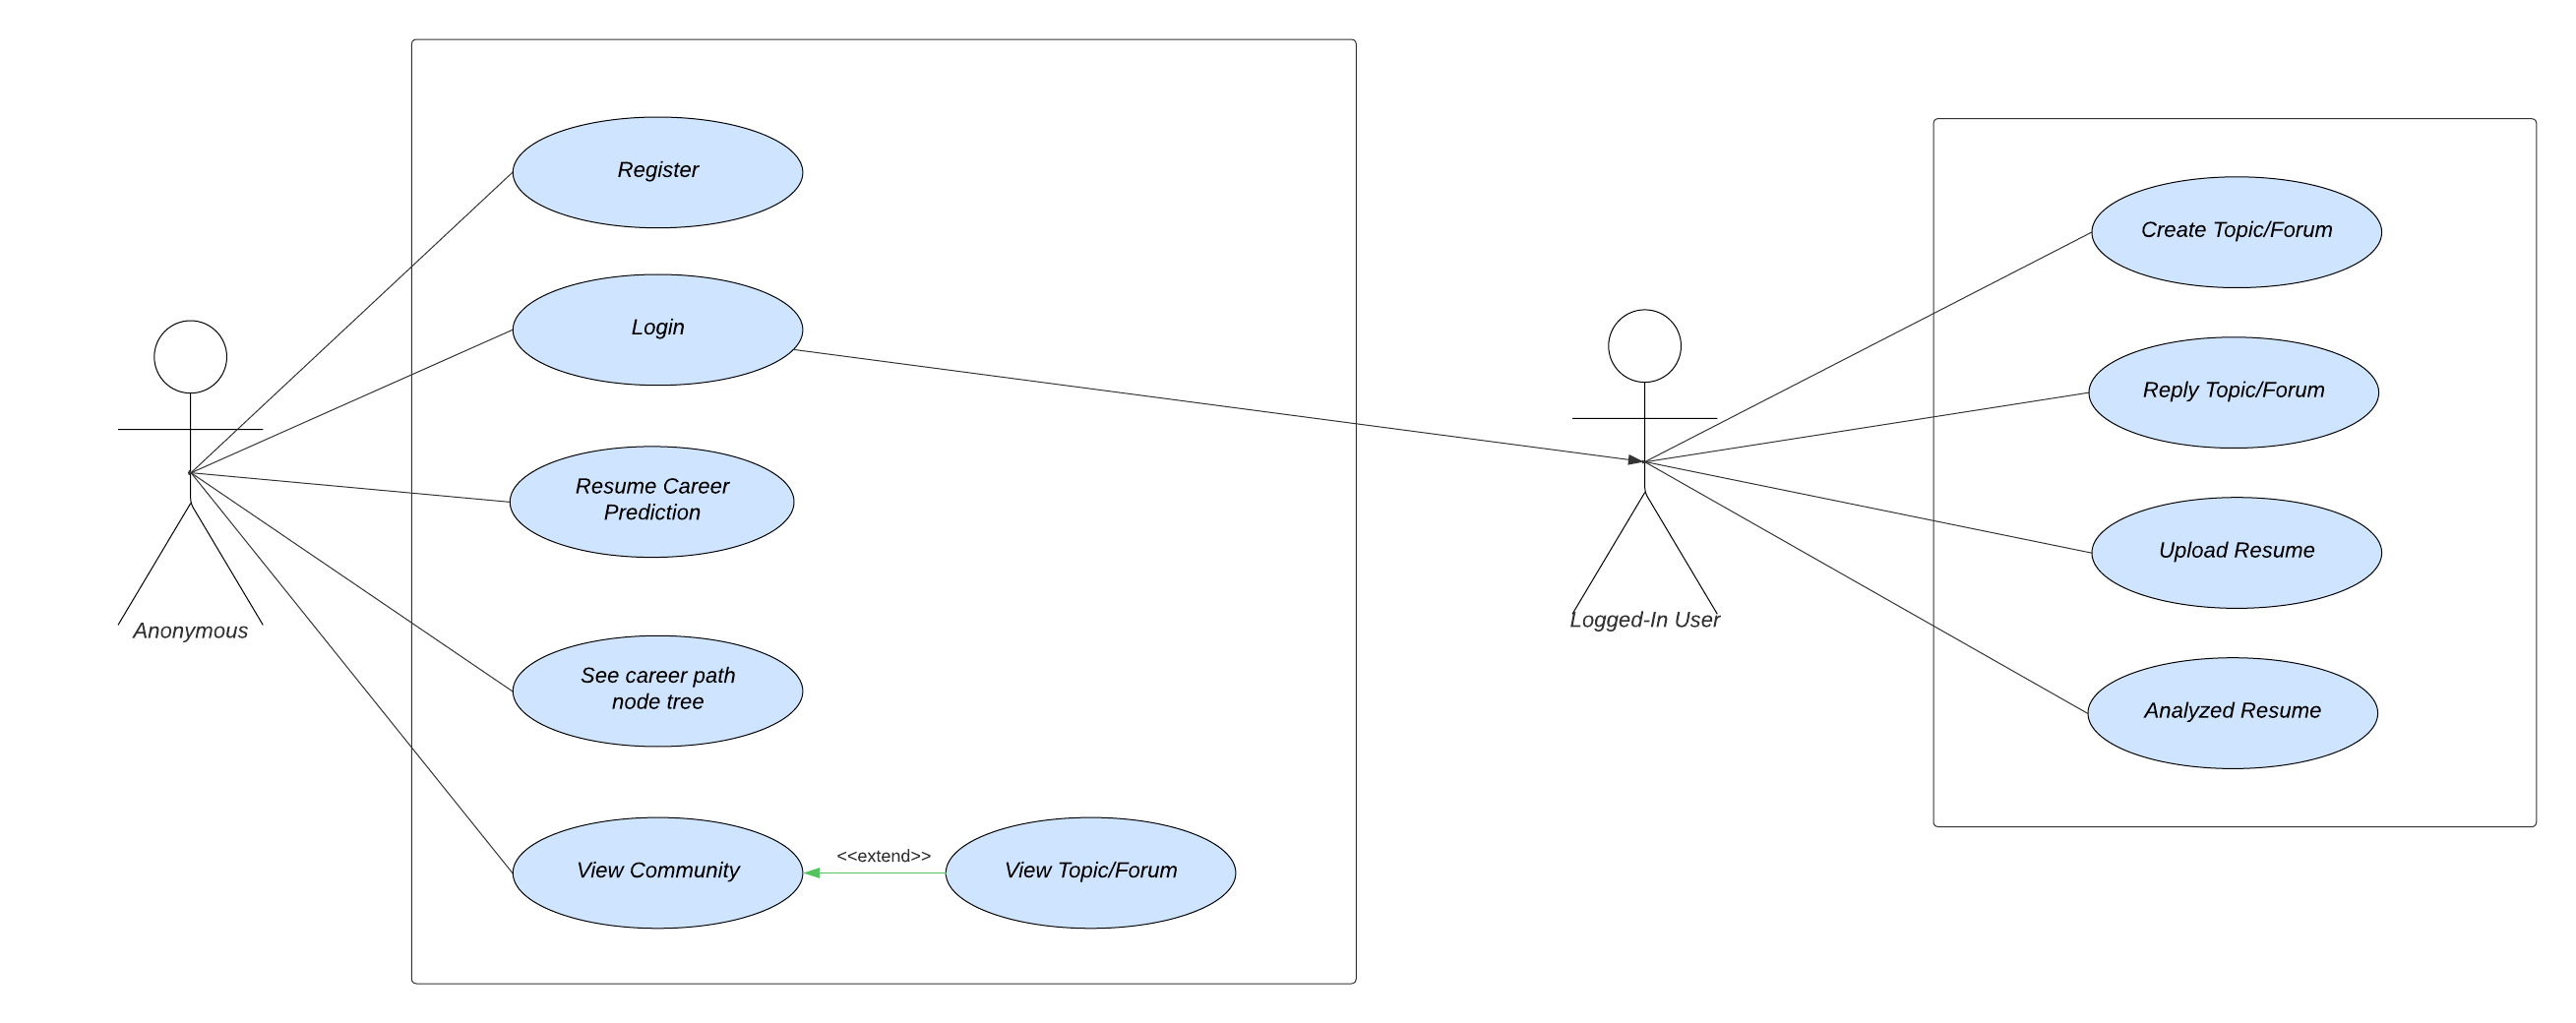
\includegraphics[width=10cm]{./figure/figure_usecase.png}}
    \caption{Use Case Diagram}\label{fig:model8}
\end{figure}
\subsection{Use Case Narrative}
\subsubsection{Resume Career Prediction}
\begin{table}[!h]
    % \centering
    \begin{tabular}{|l|l|} \hline
        Actor                 & Anonymous                                       \\ \hline
        Goal                  & ต้องการทราบถึงอาชีพที่เหมาะสมกับตนเอง                 \\ \hline
        Precondition          & -                                               \\ \hline
        Main success scenario & 1. ผู้ใช้ขอคำแนะนำอาชีพที่เหมาะสมกับตนเอง                \\
                              & 2. ระบบถามข้อมูลของผู้ใช้                            \\
                              & 3. ผู้ใช้กรอกข้อมูล                                  \\
                              & 4. ระบบถามเพื่อยืนยันการกรอกข้อมูล                    \\
                              & 5. ผู้ใช้ยืนยันการกรอกข้อมูล                           \\
                              & 6. ระบบแสดงอาชีพที่เหมาะสมกับผู้ใช้                    \\ \hline
        Extensions (a)        & 5a. ผู้ใช้กรอกข้อมูลไม่ครบ                            \\
                              & 6a. ระบบขึ้นเตือนว่าผู้ใช้ยังกรอกข้อมูลไม่ครบ              \\
                              & 7a. กลับไปที่ขั้นตอนที่ 3                              \\ \hline
        Postcodition          & ระบบแนะนำให้ผู้ใช้ไปวิเคราะห์ข้อมูลเชิงลึกของอาชีพที่ได้แนะนำไป \\ \hline
    \end{tabular}
\end{table}

\subsubsection{See career path node tree}
\begin{table}[!h]
    % \centering
    \begin{tabular}{|l|l|} \hline
        Actor                 & Anonymous                                              \\ \hline
        Goal                  & ต้องการดูแผนผังสายอาชีพ                                    \\ \hline
        Precondition          & ผู้ใช้กำลังดูแผนผังรวมของสายอาชีพ                              \\ \hline
        Main success scenario & 1. ใช้เลือกอาชีพที่ต้องการจะดู                                \\
                              & 2. ระบบแสดงรายละเอียดย่อยเป็นรูปแบบแผนผังของสายอาชีพที่ผู้ใช้เลือก \\ \hline
        Extensions (a)        & 1a. ผู้ใช้ยังไม่ได้เลือกอาชีพที่ต้องการจะดู                        \\
                              & 2a. ระบบขึ้นเตือนว่าผู้ใช้ยังไม่ได้เลือกอาชีพที่ต้องการดู              \\
                              & 3a. กลับไปที่ขั้นตอนที่ 1                                     \\ \hline
        Postcodition          & -                                                      \\ \hline
    \end{tabular}
\end{table}

\subsubsection{View Community}
\begin{table}[!h]
    % \centering
    \begin{tabular}{|l|l|} \hline
        Actor                 & Anonymous                              \\ \hline
        Goal                  & ต้องการดูรายการของกระทู้ต่าง ๆ ในชุมชน       \\ \hline
        Precondition          & ผู้ใช้กำลังดูประเภทของกระทู้                   \\ \hline
        Main success scenario & 1. ผู้ใช้เลือกประเภทของกระทู้                \\
                              & 2. ระบบแสดงรายการของกระทู้ประเภทที่ผู้ใช้เลือก \\ \hline
        Extensions (a)        & -                                      \\ \hline
        Postcodition          & -                                      \\ \hline
    \end{tabular}
\end{table}

\subsubsection{View Topic/Forum}
\begin{table}[!h]
    % \centering
    \begin{tabular}{|l|l|} \hline
        Actor                 & Anonymous                                        \\ \hline
        Goal                  & ต้องการดูรายละเอียดของกระทู้                          \\ \hline
        Precondition          & ผู้ใช้กำลังดูรายการของกระทู้ที่อยู่ในชุมชน (กระทู้ประเภทไหนก็ได้) \\ \hline
        Main success scenario & 1. ผู้ใช้เลือกกระทู้ที่ต้องการดูรายละเอียด                  \\
                              & 2. ระบบแสดงรายละเอียดของกระทู้ผู้ใช้เลือก               \\ \hline
        Extensions (a)        & -                                                \\ \hline
        Postcodition          & -                                                \\ \hline
    \end{tabular}
\end{table}

\subsubsection{Create Topic/Forum}
\begin{table}[!h]
    % \centering
    \begin{tabular}{|l|l|} \hline
        Actor                 & Logged-in User                                   \\ \hline
        Goal                  & ต้องการสร้างกระทู้                                   \\ \hline
        Precondition          & ผู้ใช้กำลังดูรายการของกระทู้ที่อยู่ในชุมชน (กระทู้ประเภทไหนก็ได้) \\ \hline
        Main success scenario & 1. ผู้ใช้เลือกกระทู้ที่ต้องการดูรายละเอียด                  \\
                              & 2. ระบบถามรายละเอียดภายในกระทู้                     \\
                              & 3. ผู้ใช้กรอกรายอะเอียดภายในกระทู้                     \\
                              & 4. ระบบถามเพื่อยืนยันการลงกระทู้                       \\
                              & 5. ผู้ใช้ยืนยันการลงกระทู้                              \\
                              & 6. ระบบสร้างและแสดงกระทู้ของผู้ใช้                     \\ \hline
        Extensions (a)        & 5a. ผู้ใช้กรอกข้อมูลไม่ครบ                             \\
                              & 6a. ระบบขึ้นเตือนว่าผู้ใช้ยังกรอกข้อมูลไม่ครบ               \\
                              & 7a. กลับไปที่ขั้นตอนที่ 3                               \\ \hline
        Postcodition          & กระทู้ของผู้ใช้แสดงอยู่ในชุมชน                           \\ \hline
    \end{tabular}
\end{table}

\subsubsection{Reply Topic/Forum}
\begin{table}[!h]
    % \centering
    \begin{tabular}{|l|l|} \hline
        Actor                 & Logged-in User                                   \\ \hline
        Goal                  & ต้องการแสดงความคิดเห็นในกระทู้                        \\ \hline
        Precondition          & ผู้ใช้กำลังดูรายการของกระทู้ที่อยู่ในชุมชน (กระทู้ประเภทไหนก็ได้) \\ \hline
        Main success scenario & 1. ผู้ใช้เลือกส่วนที่ต้องการแสดงความคิดเห็น                \\
                              & 2. ระบบถามถึงรายละเอียดความคิดเห็น                   \\
                              & 3. ผู้ใช้กรอกความคิดเห็น                              \\
                              & 4. ระบบถามเพื่อยืนยันการแสดงความคิดเห็น                \\
                              & 5. ผู้ใช้ยืนยันการแสดงความคิดเห็น                       \\
                              & 6. ระบบสร้างและแสดงความคิดเห็นของผู้ใช้ในกระทู้          \\ \hline
        Extensions (a)        & 4a. ผู้ใช้ยังไม่ได้กรอกความคิดเห็น                       \\
                              & 5a. ระบบขึ้นเตือนว่าผู้ใช้ยังไม่ได้กรอกความคิดเห็น           \\
                              & 6a. กลับไปที่ขั้นตอนที่ 3                               \\ \hline
        Postcodition          & ความคิดเห็นของผู้ใช้แสดงอยู่ในกระทู้                      \\ \hline
    \end{tabular}
\end{table}

\subsubsection{Upload Resume}
\begin{table}[!h]
    % \centering
    \begin{tabular}{|l|l|} \hline
        Actor                 & Logged-in User                                  \\ \hline
        Goal                  & ต้องการอัพโหลดเรซูเม่                               \\ \hline
        Precondition          & ผู้ใช้กำลังอยู่ดูข้อมูลส่วนตัวของตนเอง                      \\ \hline
        Main success scenario & 1. ผู้ใช้เลือกเรซูเม่ที่ต้องการอัพโหลด                    \\
                              & 2. ระบบถามเพื่อยืนยันการอัพโหลดเรซูเม่                 \\
                              & 3. ผู้ใช้ยืนยันการอัพโหลดเรซูเม่                        \\
                              & 4. ระบบอัพโหลดและแจ้งเตือนว่าอัพโหลดเรซูเม่สำเร็จ        \\ \hline
        Extensions (a)        & 3a. ผู้ใช้เลือกเรซูเม่ที่ต้องการอัพโหลด                   \\
                              & 4a. ระบบขึ้นเตือนว่าผู้ใช้ยังไม่ได้เลือกเรซูเม่ที่ต้องการอัพโหลด \\
                              & 5a. กลับไปที่ขั้นตอนที่ 1                              \\ \hline
        Postcodition          & เรซูเม่แสดงอยู่ในข้อมูลส่วนตัวของผู้ใช้                    \\ \hline
    \end{tabular}
\end{table}

\subsubsection{Analyzed Resume}
\begin{table}[!h]
    % \centering
    \begin{tabular}{|l|l|} \hline
        Actor                 & Logged-in User                  \\ \hline
        Goal                  & ต้องการดูข้อมูลเชิงลึกของอาชีพ         \\ \hline
        Precondition          & ผู้ใช้ต้องมีอาชีพที่ระบบแนะนำให้          \\ \hline
        Main success scenario & 1. ผู้ใช้เลือกอาชีพที่ต้องการดูข้อมูลเชิงลึก \\
                              & 2. ระบบแสดงข้อมูลเชิงลึกของอาชีพ     \\ \hline
        Extensions (a)        & 1a. ผู้ใช้ต้องวิเคราะห์อาชีพใหม่        \\
                              & 2a. ระบบถามถึงข้อมูลของผู้ใช้         \\
                              & 3a. ผู้ใช้กรอกข้อมูลใหม่              \\
                              & 4a. ผู้ใช้ยืนยันการกรอกข้อมูล          \\
                              & 5a. ระบบแสดงอาชีพที่เหมาะสมกับผู้ใช้   \\
                              & 6a. กลับไปที่ขั้นตอนที่ 1              \\ \hline
        Postcodition          & -                               \\ \hline
    \end{tabular}
\end{table}

\section{สถาปัตยกรรมของระบบ}
\begin{figure}[!h]\centering
    \setlength{\fboxrule}{0.2mm} % can define this in the preamble
    \setlength{\fboxsep}{0.5cm}
    \fbox{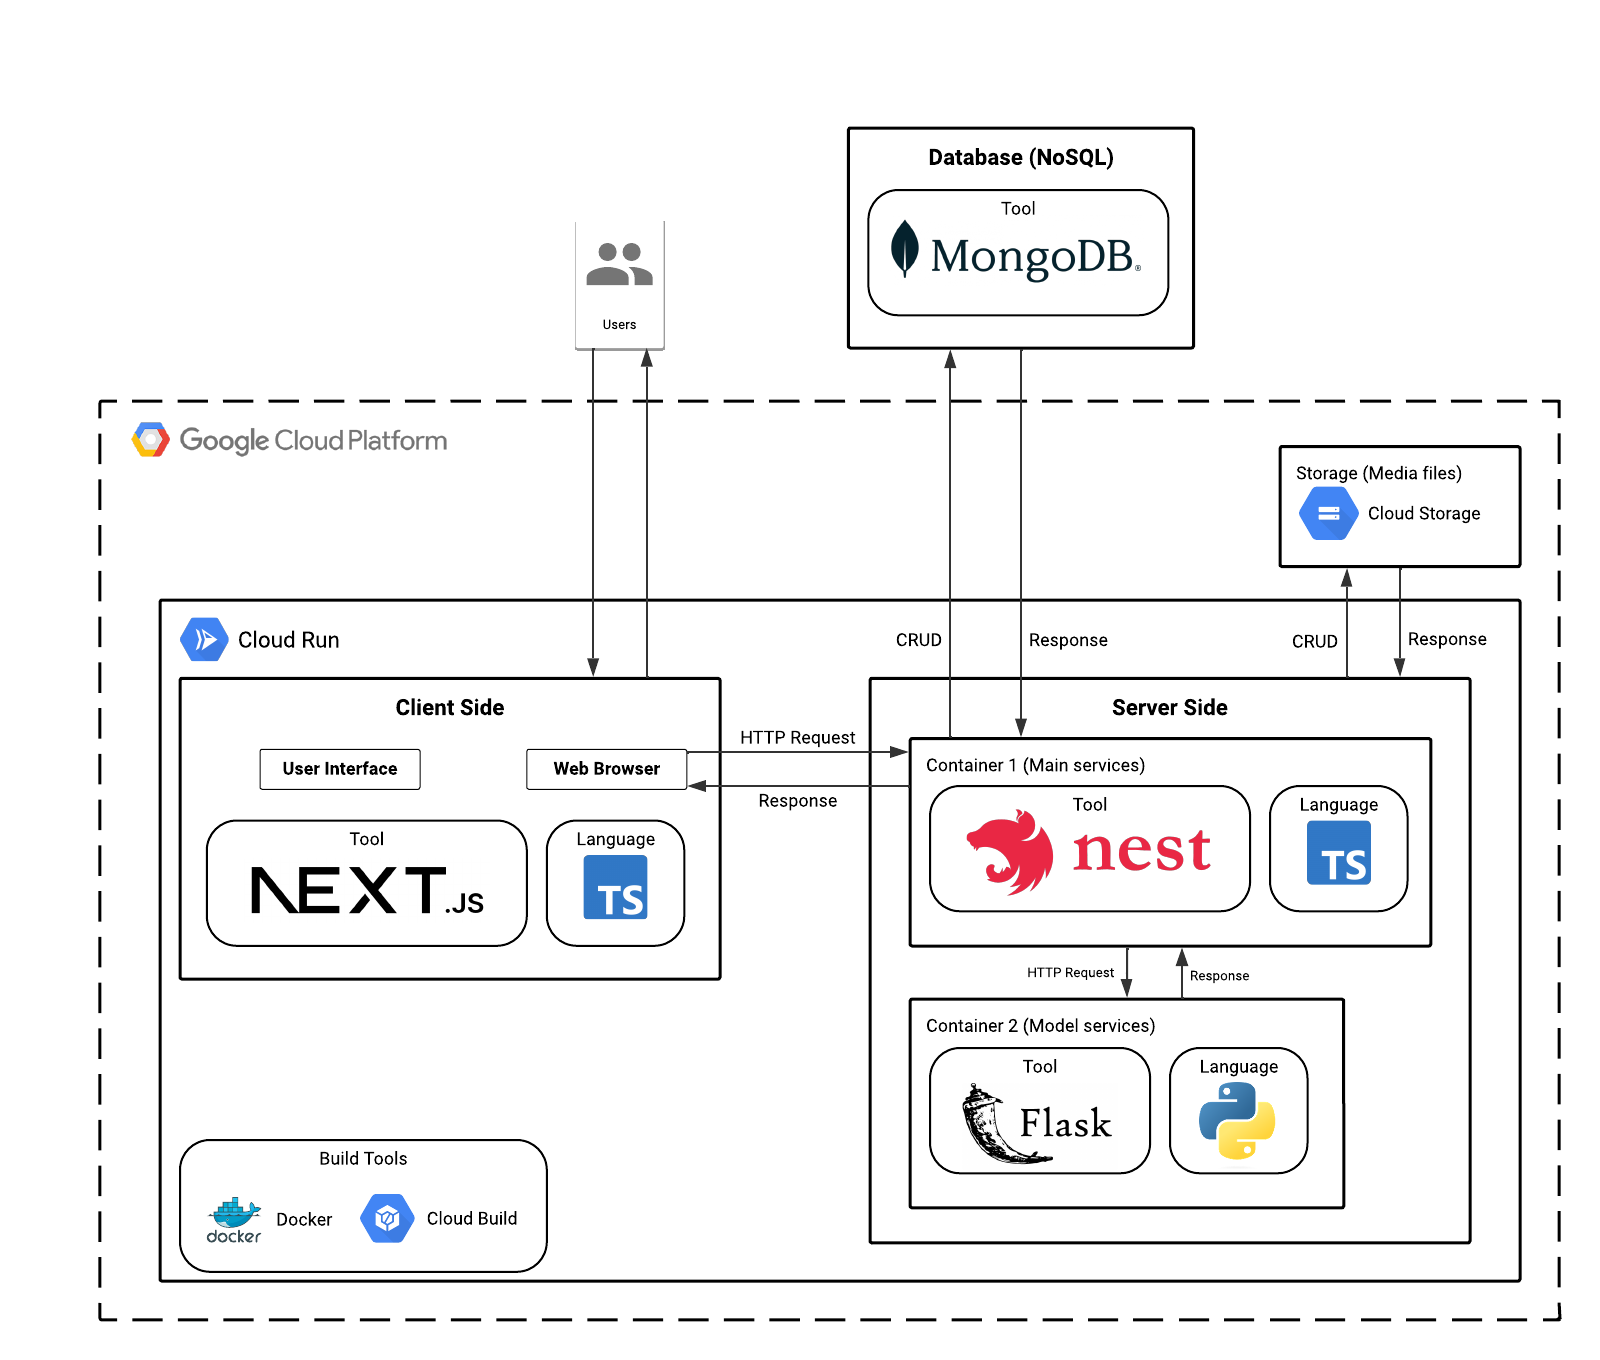
\includegraphics[width=10cm]{./figure/figure_system_architecture.png}}
    \caption{System Architecture}\label{fig:model4}
\end{figure}
จากแผนผังสถาปัตยกรรมระบบ เราได้ใช้บริการ Google Cloud เป็นหลักเนื่องจากสะดวกต่อการ scaling ในอนาคต สามารถจัดการและเปลี่ยนแปลงเวอร์ชันได้รวดเร็วระหว่างการพัฒนา โดยสถาปัตยกรรมแต่ละส่วนมีหน้าที่หลักดังนี้

\subsection{ส่วนผู้ใช้ (Client-Side)}
รับผิดชอบในการติดต่อปฏิสัมพันธ์กับผู้ใช้ แสดง user interface ผ่านทาง web browser และเชื่อมต่อกับ server เพื่อขอข้อมูลและใช้บริการต่าง ๆ

\subsection{ส่วนเซิร์ฟเวอร์ (Server-Side)}
รับผิดชอบในการจัดการตรรกะและระบบคำนวณต่าง ๆ ทุกรูปแบบและส่งกลับไปให้ผู้ใช้ โดยทางคณะู้จัดทำได้แบ่งระบบ server เป็นสองบริการหลัก ประกอบด้วย
\newline
1. บริการหลัก (Main services)
\newline
บริการที่จะติดต่อกับผู้ใช้โดยตรงเพียงหนึ่งเดียว มีหน้าที่ในการจัดการทุกคำขอจากผู้ใช้ผ่านทาง API (Application Programming Interfaces) เช่น ดึงข้อมูลจากฐานข้อมูล คำนวณค่าต่าง ๆ และติดต่อกับบริการอื่น ๆ
\newline
2. บริการโมเดล (Model services)
\newline
บริการสำหรับใช้คำนวณเกี่ยวกับปัญญาประดิษฐ์ของทางคณะผู้จัดทำเท่านั้น เนื่องจากกินทรัพยากรสูง การแยกบริการออกมาจากบริการหลักจึงสามารถดูแลและจัดการได้ง่ายกว่า โดยจะรับค่ามาจากส่วนบริการหลักและส่งค่ากลับไปให้

\newpage

\section{Site Map}
\begin{figure}[h]\centering
    \setlength{\fboxrule}{0.2mm} % can define this in the preamble
    \setlength{\fboxsep}{0.5cm}
    \fbox{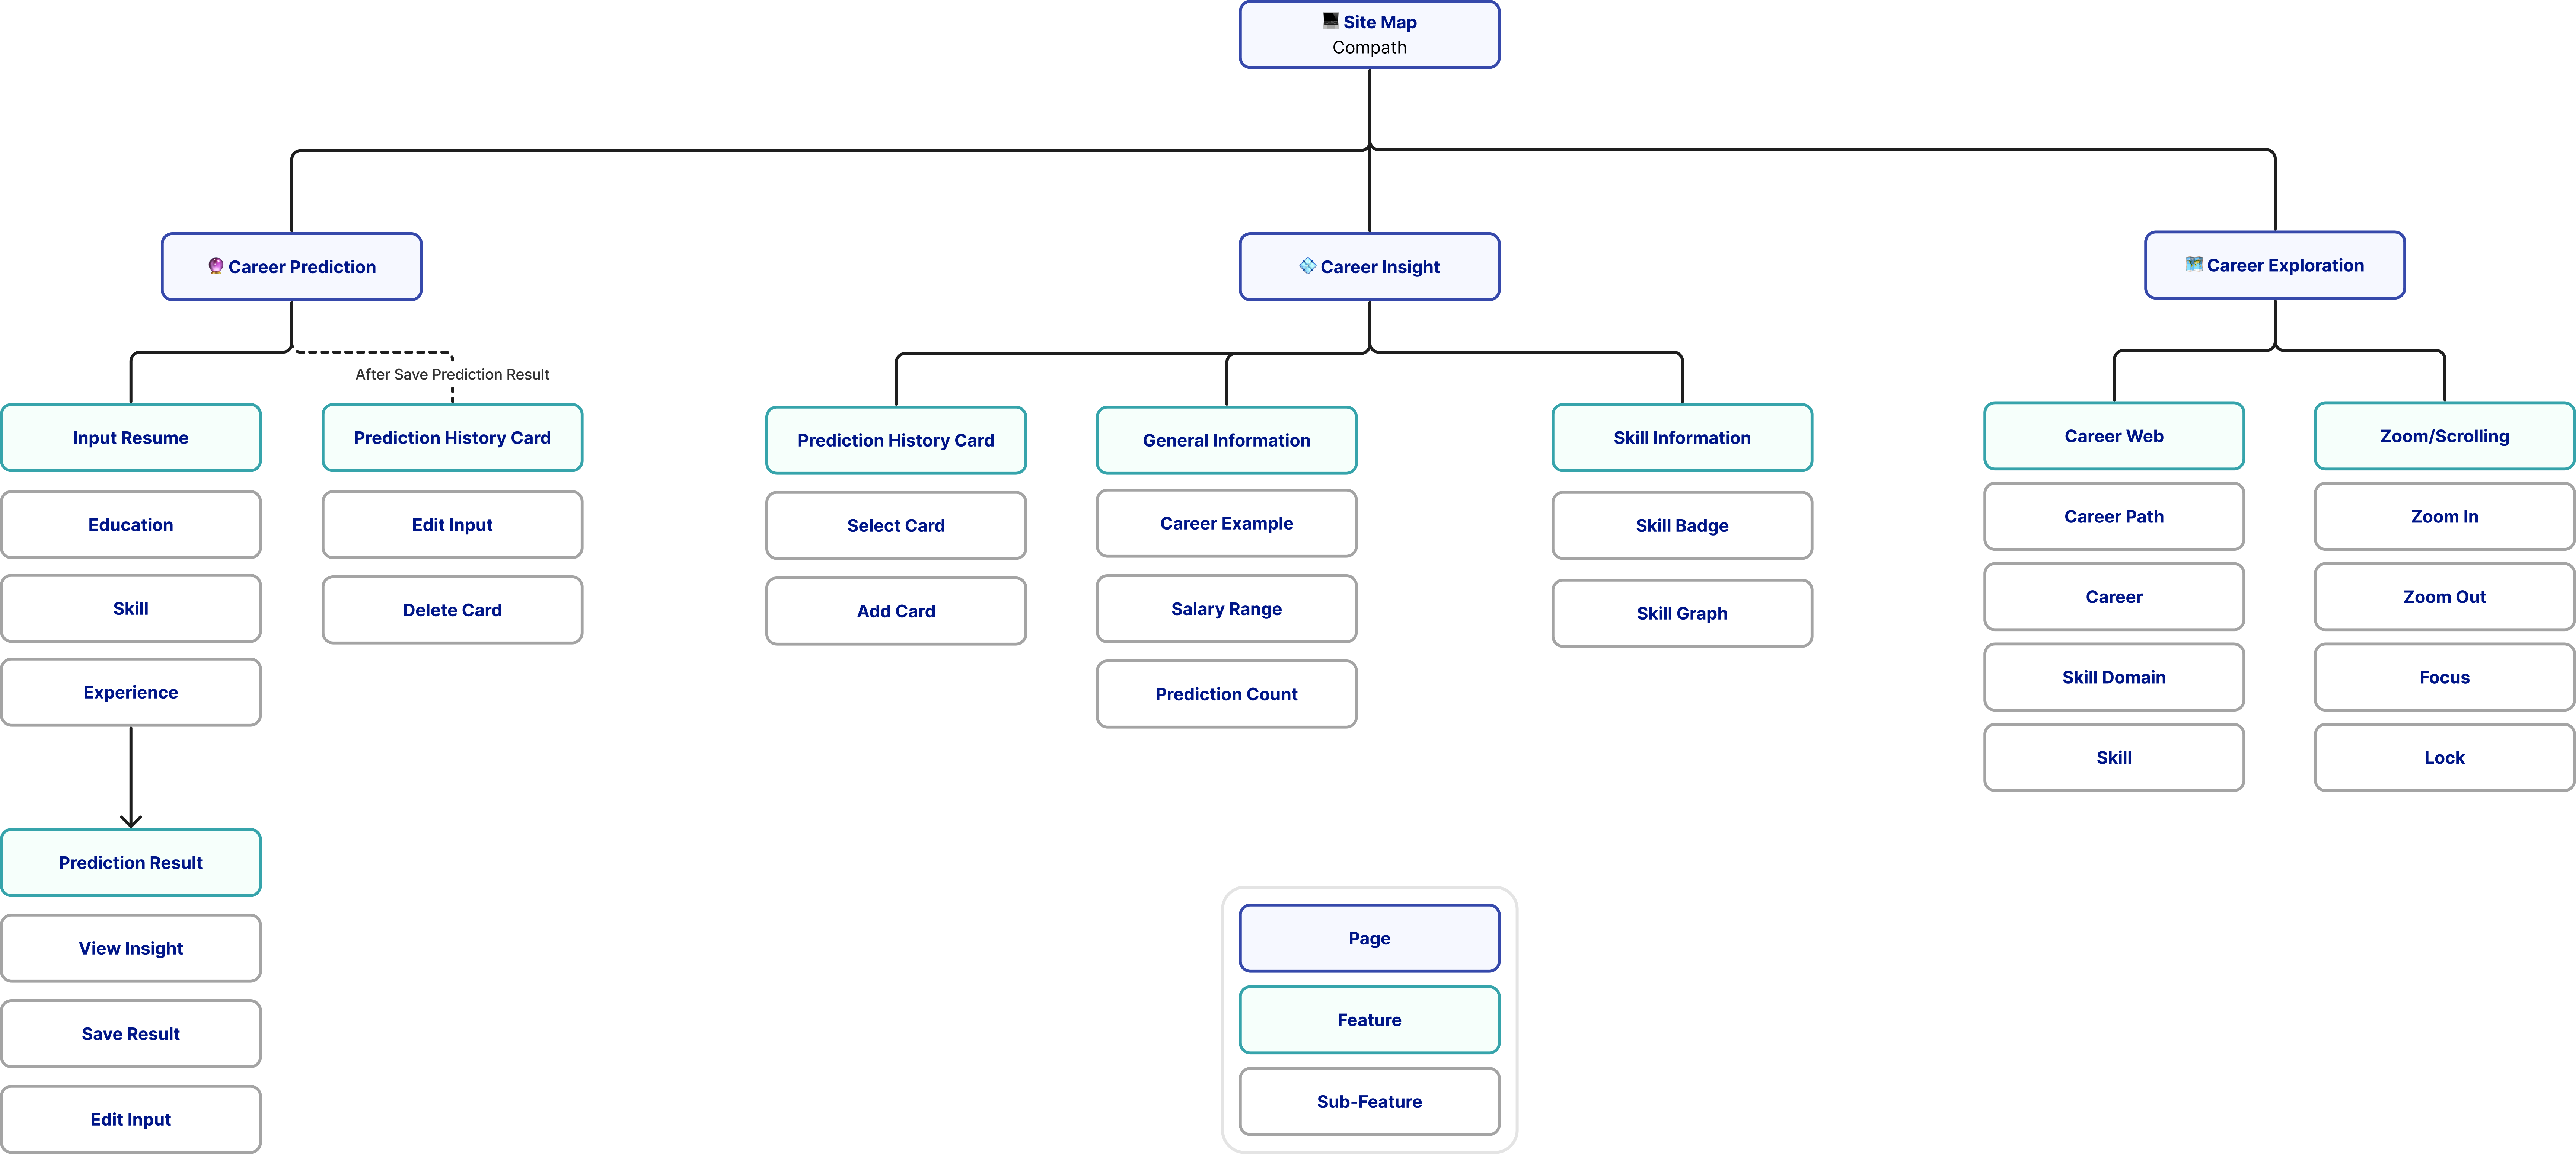
\includegraphics[width=10cm]{./figure/figure_siteMap.png}}
    \label{fig:siteMap}
\end{figure}

\section{Navigation Map}
\begin{figure}[h]\centering
    \setlength{\fboxrule}{0.2mm} % can define this in the preamble
    \setlength{\fboxsep}{0.5cm}
    \fbox{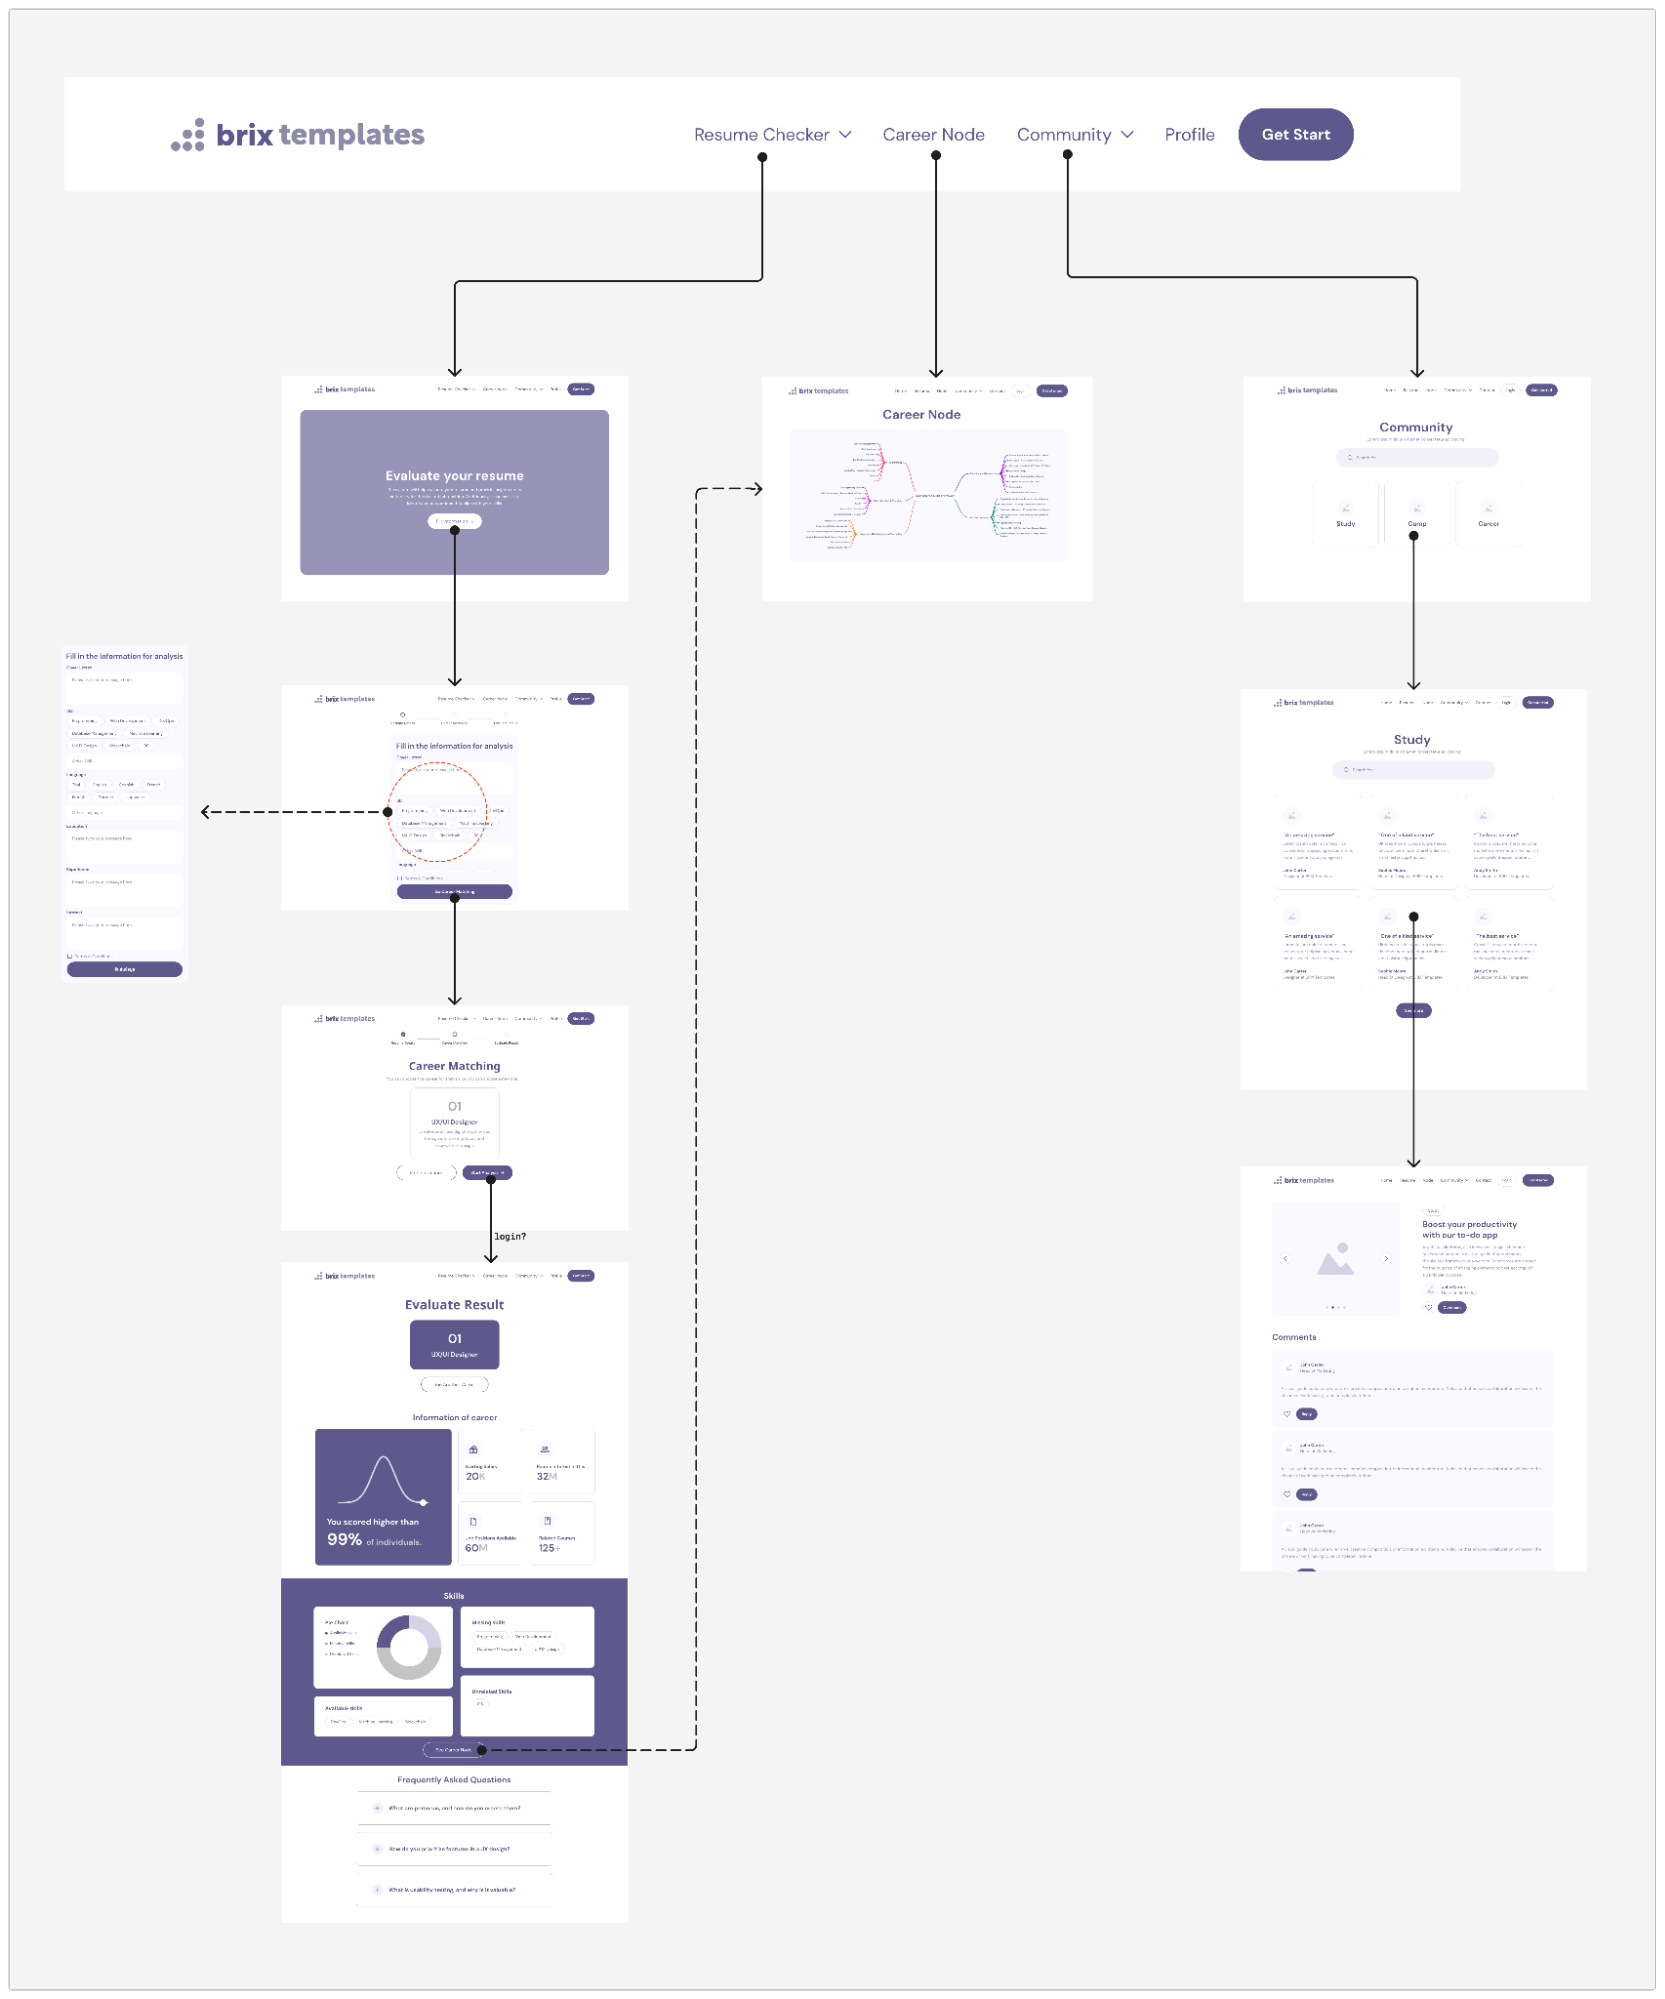
\includegraphics[width=10cm]{./figure/figure_navMap.png}}
    \label{fig:navMap}
\end{figure}

\section{ขั้นตอนการพัฒนาโมเดล}
\subsection{การรวบรวมข้อมูล (Get Data)}
ทางคณะผู้จัดทำได้เลือกนำชุดข้อมูล Updated Resume Dataset \cite{dataset} จาก Kaggle ซึ่งเป็นชุดข้อมูล
ที่ประกอบไปด้วยอาชีพทั้งหมด 25 หมวด และรายละเอียดภายในเรซูเมของแต่ละอันที่จะแตกต่างกันไปในแต่ละอัน ซึ่งมีเรซูเม
ทั้งหมด 962 เล่ม
\begin{figure}[h]\centering
    \setlength{\fboxrule}{0.2mm} % can define this in the preamble
    \setlength{\fboxsep}{0.5cm}
    \fbox{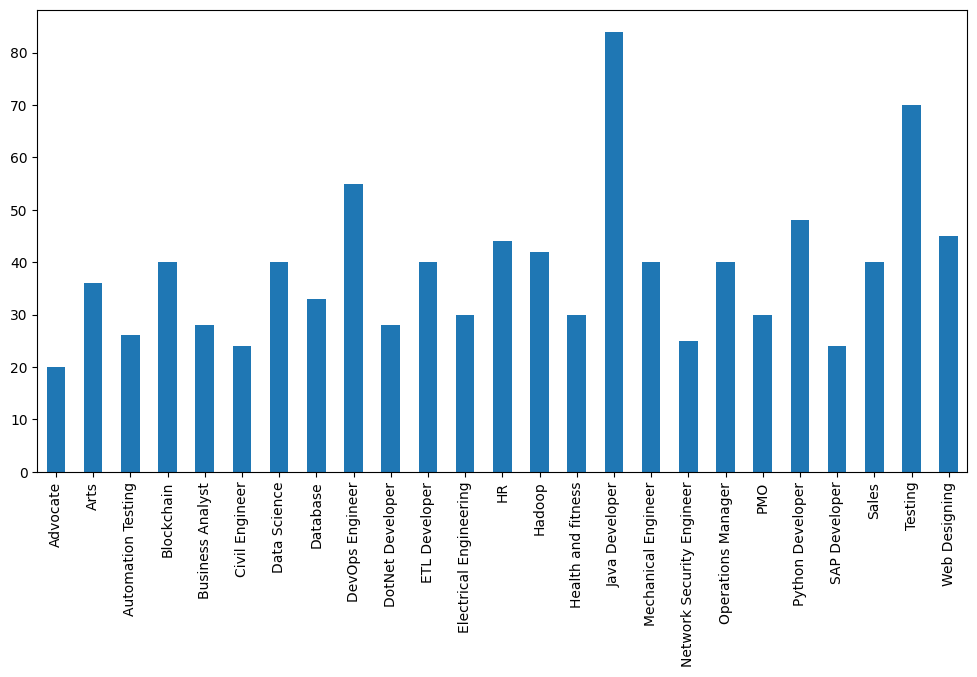
\includegraphics[width=10cm]{./figure/figure_datasetCategory.png}}
    \caption{จำนวนของเรซูเมในแต่ละหมวดอาชีพ}\label{fig:datasetCategory}
\end{figure}
\begin{figure}[h]\centering
    \setlength{\fboxrule}{0.2mm} % can define this in the preamble
    \setlength{\fboxsep}{0.5cm}
    \fbox{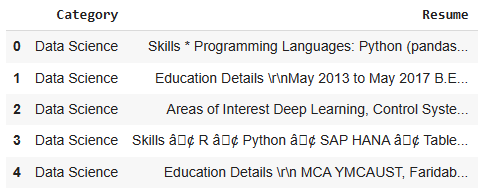
\includegraphics[width=10cm]{./figure/figure_datasetData.png}}
    \caption{ลักษณะข้อมูลของชุดข้อมูล}\label{fig:datasetData}
\end{figure}
\par ซึ่งทางคณะผู้จัดทำ จำเป็นต้องทำการเตรียมข้อมูลที่เหมาะสมเพื่อให้โมเดลมีประสิทธิภาพ

\subsection{การเตรียมข้อมูล (Clean, Prepare and Manipulate Data)}
หลังจากที่ทางคณะผู้จัดทำได้ทำการสำรวจชุดข้อมูล ทำให้พบว่ารายละเอียดของเรซูเมยังไม่สามารถนำไปใช้ได้ทันที
เนื่องจากข้อมูลเรซูเม ได้มีตัวอักษรพิเศษรวมอยู่เป็นจำนวนมาก เช่น \^a, €, ¢, \textbackslash r, \textbackslash n
รวมไปถึงมีการใส่ลิงก์ภายนอกอีกด้วย ทางคณะผู้จัดทำจึงจำเป็นที่จะต้องทำให้ตัวหนังสือภายในเรซูเม เป็นเพียงตัวอักษรปกติเท่านั้น
\par เนื่องจากทางคณะผู้จัดทำเล็งเห็นกลุ่มเป้าหมายเป็นนักศึกษาวิศวกรรมคอมพิวเตอร์ มจธ. จึงจำเป็นที่ต้องเลือกเฉพาะข้อมูลที่เป็น
Software Engineer, Designer, Data, Security, Cloud Management ซึ่งเราจำเป็นที่จะต้อง
ลบบางหมวดอาชีพ และทำการรวมบางอาชีพเข้าด้วยกัน
\par และเพื่อให้โมเดลสามารถที่จะเข้าใจภาษาของมนุษย์ได้ คณะผู้จัดทำจึงได้ใช้อัลกอริทึมในการแปลผลภาษา
Term Frequency Inverse Document Frequency (TF-IDF)

\subsection{การเทรนโมเดล (Train Model)}
หลังจากที่ทางคณะผู้จัดทำได้ทำการเตรียมข้อมูลสำเร็จแล้ว คณะผู้จัดทำก็ได้ทำโมเดลขึ้นมาทั้งหมด 2 โมเดลเพื่อเปรียบเทียบ
ซึ่งเป็นโมเดลสำหรับการจัดหมวดหมู่ ได้แก่
\begin{enumerate}
    \item Navie Bayes Classification
    \item Long Short Term Memory (LSTM)
    \begin{itemize}
        \item Embedding layer              | max input dimension is 10,000 and embedding dimension size is 100
        \item Bidirectional LSTM 128 units | dropout rate 40\%
        \item Bidirectional LSTM 64 units  | dropout rate 40\%
        \item Dense layer 25 units         | softmax as activation function
    \end{itemize}
\end{enumerate}
\par และคณะผู้จัดทำก็ทำการใส่ข้อมูลที่เตรียมเอาไว้เพื่อทำการเทรนโมเดล โดยที่โมเดลจะทำการทำนายว่าข้อมูลเรซูเมที่ใส่เข้าไป
เป็นอาชีพใดจากทั้งหมด 5 อาชีพ (Software Engineer, Designer, Data, Security, Cloud Management) ซึ่ง
สามารถแสดงผลออกมาเป็นความน่าจะเป็นของแต่ละสายอาชีพได้

\subsection{การทดสอบข้อมูล (Test Data)}
หลังจากที่คณะผู้จัดทำได้เทรนโมเดลจนสำเร็จแล้ว ก็ได้ลองนำเรซูเมของคณะผู้จัดทำมาลองกับโมเดล ซึ่งผลลัพธ์ที่ได้ก็ค่อนข้างน่าพอใจ
คาดว่าเนื่องจากมีสายอาชีพที่ต้องทำนายค่อนข้างน้อย ทำให้มีโอกาสที่จะทำนายได้ถูกต้องค่อนข้างสูง

\subsection{การพัฒนาโมเดล (Improve)}
ทางคณะผู้จัดทำคาดหวังว่าจะพัฒนาโมเดลได้ด้วยการหาชุดข้อมูลสำหรับการเทรนมากขึ้นกว่านี้ และเพิ่มจำนวน Epoch สำหรับการเทรน
Long Short Term Memory (LSTM) ที่มากกว่านี้ และคาดหวังว่าในอนาคตจะมีสายอาชีพที่ทำการทำนายเพิ่มมากขึ้นกว่านี้

% \emph{หัวข้อต่าง ๆ ในแต่ละบทเป็นเพียงตัวอย่างเท่านั้น หัวข้อที่จะใส่ในแต่ละบทขึ้นอยู่กับโปรเจคของนักศึกษาและอาจารย์ที่ปรึกษา}


% ตัวอย่างการใส่อ้างอิงที่มา -> \cite{hypersense} ถ้าต้องการใส่แหล่งอ้างอิงมากกว่า 1 ให้ทำดังนี้ -> \cite{hypersense,bworld}
% Explain the design (how you plan to implement your work) of your project. Adjust the section titles below to suit the types of your work. Detailed physical design like circuits and source codes should be placed in the appendix.

% \section{ข้อกำหนดและความต้องการของระบบ}

% \section{สถาปัตยกรรมระบบ}

% \begin{table}[!h]
%     % \centering
%     \caption{test table x1}\label{tbl:symbols}
%     \begin{tabular}{@{}p{0.07\textwidth}|p{0.7\textwidth}p{0.1\textwidth}}\hline
%         \multicolumn{2}{l}{\textbf{SYMBOL}} & \textbf{UNIT}                         \\ \hline
%         $\alpha$                            & Test variable\hfill     & m$^2$       \\
%         $\lambda$                           & Interarrival rate\hfill & jobs/second \\
%         $\mu$                               & Service rate\hfill      & jobs/second \\ \hline
%     \end{tabular}
%     %\begin{tabular}{c|c} \hline
%     % $\alpha$ & $\beta$ \\ \hline
%     % $\delta$ & $\mu$ \\ \hline
%     %\end{tabular}
% \end{table}



% \section{Hardware Module 1}
% \subsection{Component 1}
% \subsection{Logical Circuit Diagram}

% \section{Hardware Module 2}
% \subsection{Component 1}
% \subsection{Component 2}

% \section{Path Finding Algorithm}

% \section{Database Design}

% \section{UML Design}

% \section{GUI Design}

% \section{การออกแบบการทดลอง}
% \subsection{ตัวชี้วัดและปัจจัยที่ศึกษา}
% \subsection{รูปแบบการเก็บข้อมูล}